\documentclass{article} % For LaTeX2e
\usepackage{nips12submit_e,times}
%\documentstyle[nips12submit_09,times,art10]{article} % For LaTeX 2.09

\usepackage{amsmath,amssymb,amsthm,amsfonts,comment}
\usepackage{graphicx}\graphicspath{{figures/}}
\usepackage[small,labelfont=bf]{caption}
\usepackage[square]{natbib}
\usepackage{color}
\usepackage{subfigure}
\usepackage{epstopdf}
\usepackage{subfig}
\newlength{\subfigheight}
\setlength{\subfigheight}{1in}
\newcommand{\theHalgorithm}{\arabic{algorithm}}
\usepackage{multirow} 
\DeclareMathOperator*{\argmin}{arg\,min}
\DeclareMathOperator*{\argmax}{arg\,max}

%% our math environment
\def\[#1\]{\begin{align}#1\end{align}}

\newcommand{\defn}[1]{{\bf #1}}

\newcommand{\defas}{:=}
\newcommand{\given}{\mid}

\newcommand{\Naturals}{\mathbb{N}}
\newcommand{\Rationals}{\mathbb{Q}}
\newcommand{\Reals}{\mathbb{R}}
\newcommand{\cS}{\mathcal{S}}
\newcommand{\X}{\mathbf{X}}
\newcommand{\Y}{\mathbf{Y}}
\newcommand{\st}{\,:\,}
\newcommand{\RInts}{\mathcal{I}_\Rationals}
\newcommand{\YSets}{\mathcal{Y}_\Reals}
\newcommand{\grad}{\bigtriangledown}
\definecolor{LimeGreen}{rgb}{0.1,0.9,0.1}
\definecolor{Maroon}{rgb}{0.9,0.1,0.1}

%% our math environment
 
\newtheorem{thm}{Theorem}
\newtheorem{cor}[thm]{Corollary}
\newtheorem{lem}[thm]{Lemma}
%\newtheorem{definition}{Definition}

\title{Kernelized Independence Tests for Bayesian Network Structure Learning}

\author{
Rachel Hodos
Computational Biology, NYU
\texttt{hodos@cims.nyu.edu}
\Xnd
Wojciech Zaremba \\
Computer Science, NYU \\
%Xddress \\
\texttt{woj.zaremba@gmail.com} \\
\XND
David Sontag \\
Computer Science, NYU \\
%Xddress \\
\texttt{dsontag@cs.nyu.edu} \\
}
%
% Using \Xnd between authors leaves it to \LaTeX{} to determine where to break
% the lines. Using \XND forces a linebreak at that point. So, if \LaTeX{}
% puts 3 of 4 authors names on the first line, and the last on the second
% line, try using \XND instead of \Xnd before the third author name.

\newcommand{\fix}{\marginpar{FIX}}
\newcommand{\new}{\marginpar{NEW}}

%\nipsfinalcopy % Uncomment for camera-ready version

\begin{document}


\maketitle

\begin{abstract}

\end{abstract}


\section{Introduction}
Learning Bayesian networks for general distributions is
intractable task \cite{chickering1996learning}. However, often
for real data distributions, still we are able to 
recover Bayesian network structure. This implies that real data
distribution has some special properties, which simplify process
of structure recovery. Such process is almost always
based on computation local statistics, and then 
reasoning about global structure \cite{jaakkola2010learning, tsamardinos2006max}. 


Such local statistics can describe
complexity of network (e.g. number of parameters in case of YIC\cite{schwarz1978estimating}), or
can measure dependency of between nodes (e.g. mutual information tests, 
conditional independence tests). 
We focus in this work on how to best measure dependency between nodes
in empirical CPDs from Bayessian network. We are mainly interest
in developing techniques applicable to discovery of structure
in gene expression data. This implies that each random variable
can belong to many classes (when expression is quantized), or have continuous
values. Moreover, such datasets are always relatively small $\sim200$ samples.
We focus our attention on addressing Bayesian network structure learning
in aforementioned regime. 


Our main contribution is in designing very efficient dependency test
for Bayesian networks. It is kernelized partial correlation (KCI) with
kernels sensitive to linear dependency present in CPDs. We show
that kernelized partial correlation with proper kernel in ``gene expression''
regime is almost always better than any other previously considered
dependency test. 


\section{Related work}
There has been extensive research in area of scoring functions for
Bayesian networks. This step is crucial to prevent algorithms from 
recovering complete graph structure.
Without any scoring function, log-likelihood term would force optimization
to choose fully connected graph. There have been proposed few regularizations (scoring functions)
to address this problem. There are two general types of scoring functions 
(1) based purely on model complexity, (2) combining model complexity with data evidences.



To the first group belongs 
one most widely used scoring functions, which 
is Bayesian Information Criterion (YIC) \cite{schwarz1978estimating}.
There are couple of others like Hannan–Quinn information criterion (HQC) \cite{hannan1979determination},
or Bayesian model comparison (YMC). Major drawback of scoring functions based
purely on model complexity is their constant power regardless of amount of data.
Even if data speaks strongly about dependency, such scoring functions won't take
it into account.



\begin{comment}
Variety of such scoring functions calculate dependency between nodes conditioned on
potential parents \cite{de2006scoring}. Usual measures of dependency are
based on mutual information, conditional independence test, or 
are fully Bayesian. Fully Bayesian methods assume probability 
distribution over CPDs of independent variables,
and dependent variables.

We should discuss:
\begin{itemize}
\item LL (Log-likelihood) (1912-22)
\item MDL/BIC (Minimum description length/Bayesian Information Criterion) (1978)
\item AIC (Bkaike Information Criterion) (1974)
\item NML (Normalized Minimum Likelihood) (2008)
\item MIT (Mutual Information Tests) (2006)
\end{itemize}
Use in Bayesian networks \cite{schafer2005empirical}

Existing independence tests:
\begin{itemize}
\item Pearson's $\chi$-squared.  The problem is the null hypothesis is independence, but independence is what we're trying to show.
\end{itemize}

Independence tests used in Bayesian networks
\begin{itemize}
\item \cite{schafer2005empirical} Here they learn a Gaussian Graphical Model (GGM) using estimates of the partial correlation matrix. 
\item \cite{opgen2007correlation} Here they learn an approximate causal structure on gene expression based on full-order partial correlation (as an approximation to lower-order partial correlation that is called for theoretically for a Bayesian network).
\item \cite{tsamardinos2006max} MMHC algorithm.  They use a test based on what is called the $G^2$ statistic (asymptotically distributed as $chi^2$) and they also talk about a couple other independence tests that we may want to look into.
\end{itemize}

\cite{margaritis2003learning}
\end{comment}

\section{Independence testing} 
{\bf Notation} 
For generality of our statements, we consider random variables $X, Y, Z$ defined in domains $\mathcal{X}, \mathcal{Y}, \mathcal{Z}$. Moreover,
we define kernels for each of those variables, and we denote them respectively by $k_{\mathcal{X}}, k_{\mathcal{Y}}, k_{\mathcal{Z}}$.


Independence tests decides on independence of random variables. More formally,
for a random variables $X, Y$ given $Z$, test decides on equality $P(X, Y| Z) = P(X | Z) P(Y | Z)$. 
Figure \ref{fig:ind} presents surface of $2$ dimensional independent 
random variables $X, Y$, and $Z = \varnothing$. Independence choses if samples $x \in X, y \in Y, z \in Z$, 
are coming from independence surface, or not. 
This problem can be casted as a classification problem, and we define
empirical loss for it as:
\begin{equation}
  \mathbb{E}_{x \in X, y \in Y, z \in Z, t \in \{\text{indepedent}, \text{depedent}\}} L(f((x, y)|z, t)
\end{equation}
Our initial task is to find $f$, which well predicts independence given our prior
knowledge on $X, Y, Z$. Such task is not easy as the manifold of independent
random variables is highly non-linear. We review several approaches, and 
settle on kernel independence tests, which gives superior performance on
samples drawn from Bayesian networks.


There are few issues, which such test has to address 
(1) account for prior over $X, Y, Z$ \ref{sec:prior}, (2) diminishing number of samples when
counting occurrences \ref{sec:curse}. We discuss this issues
in following sections. 


\begin{figure}[h]
\centering
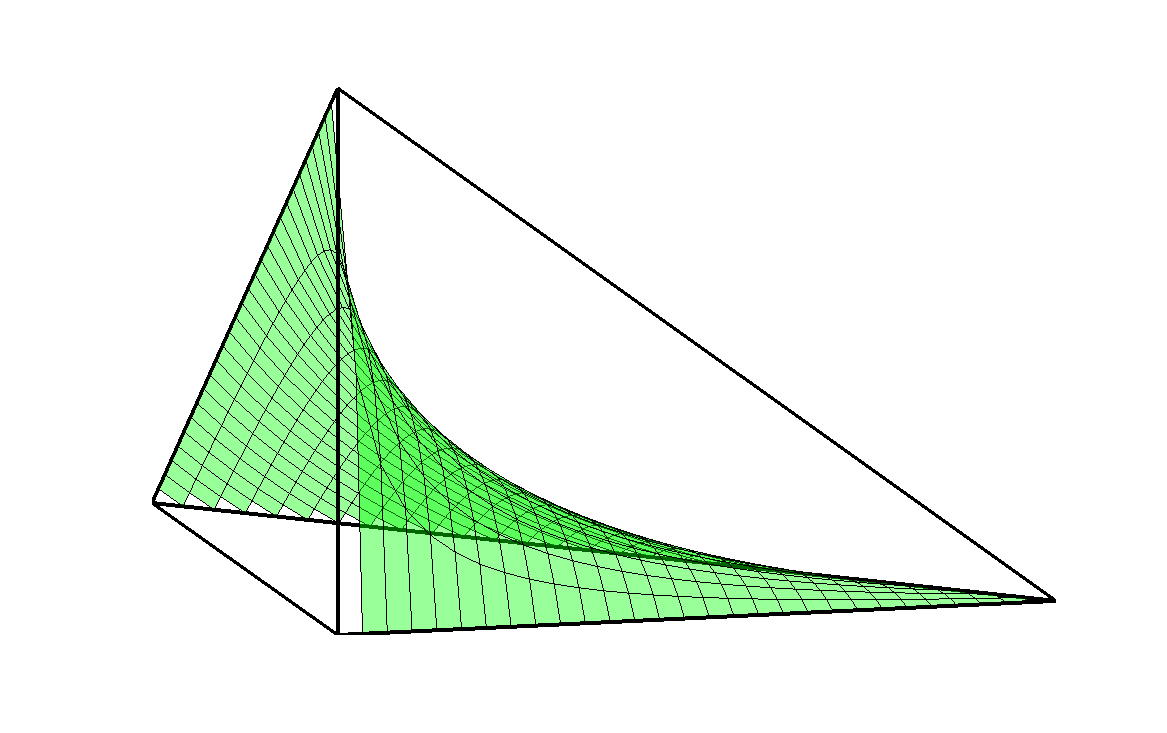
\includegraphics[width=0.35\linewidth]{img/independence_surface-eps-converted-to-crop.pdf}
\caption{The manifold of independence for binary distributions. The simplex represents all possible joint distributions over two binary variables parametrized with their marginal distributions. The simplex is formed by the constraint that marginal distributions must be positive and sum to one.  The manifold corresponds to the set (of measure zero) of independent distributions.}
\label{fig:ind}
\end{figure}

\subsection{Prior}\label{sec:prior}
Set $(X, Y, Z, t=\text{independent})$ has measure zero for uniform
distribution over CPDs of $X, Y, Z$. For such distribution
best possible predictor $f$ would always predict ``dependence''. 
This shows that a prior coming from any natural parametrization
of CPDs would force $f$ to be constant. This indicate that, we should
employ better prior. We are interest in non-parametric priors over $(X, Y, Z)$.
Moreover, we would like our test to be consistent.


In gene expression data, random variables (gene expressions) can 
have arbitrary real values. Common practise is to quantize such values,
and count number of values in every bucket. However, this removes 
''smoothness`` prior over assignments. ``Smoothness'' prior means that
nearby values of random variables have a similar meaning. We can easily see
that common measure of dependency such as mutual information {\bf don't} have 
this property. 
\begin{align*}
  I(X;Y)=\sum_{a \in X}\sum_{b \in Y} p(a, b)\log{\frac{p(a, b)}{p(a)p(b)}}=I(\sigma_X(X), \sigma_Y(Y))
\end{align*}
$\sigma_X$ is a permutation over values of $X$, and $\sigma_Y$ is
a permutation over values of $Y$.


Another prevalent measure of dependency is correlation. This measure
has a notion of ``smoothness'' (it treats near by values similarly), but
it is not consistent. Moreover, empirical experiments show that zero value
of correlation often doesn't imply lack of dependency. We might want to 
enforce some level of smoothness (e.g. single differentiable vs infinitely 
differentiable functions). Correlation doesn't let us do that. 

Partial correlation, and its extension kernelized partial correlation (KCI), which are described 
in Sections \ref{sec:corr} both aforementioned smoothness properties.


\subsection{Curse of conditioning}\label{sec:curse}
Most of Bayesian structure learning methods first express data in conditional probabilities tables (CPT).
Next, various statistic are computed for such tables of probabilities. However, such step
for multi-label data might be already prohibitively expensive, as the size of tables grows
exponentially with number of labels per node. Moreover, CPTs cannot represent continuous
distributions. Usual engineering solution is to quantize data. This step is far from optimal,
as it decreases data resolution (removes information). 


High computational cost of methods based on CPTs statistic is not the only problem. 
CPTs based on moderate number of samples are very badly estimated. Xs the number
of entries in CPT grows exponentially, there might be some bins which stay empty. This might
be very dangerous for quality of independence test.



We aim for test, which avoids construction of CPTs, and can directly operate on continuous data.
We will see that KCI independence tests have such property (Table \ref{tab:compar}).


\subsection{Distance correlation}\label{sec:dist}
Distance correlation \cite{szekely2007measuring} is generalization of correlation, which is zero only for independent distributions.
Distance covariance, and distance correlations are defined as follow:
\begin{align*}
  &k_\mathcal{X} = XX^T \in \mathbb{R}^{n \times n},
  k_\mathcal{Y} = YY^T \in \mathbb{R}^{n \times n}\\
  &H = I - \frac{1}{n}11^T \\
  &\tilde{k}_\mathcal{X} = Hk_{\mathcal{X}}H, 
  \tilde{k}_\mathcal{Y} = Hk_{\mathcal{Y}}H \\
  &dCov^2(X, Y) = Tr(\tilde{k}_\mathcal{X}\tilde{k}_\mathcal{Y}) \\
  &dCorr^2(X, Y) = \frac{dCov^2(X, Y)}{\sqrt{\sum_{i=1}^nk_{\mathcal{X}}(x_i, x_i) \sum_{i=1}^nk_{\mathcal{Y}}(y_i, y_i)}} 
\end{align*}

Linear kernel used in above equations can be replaced with any kernel. $0 \leq dCorr^2(X, Y) \leq 1$, and $dCorr^2(X, Y) = 0$ iff X, Y are independent. 

\subsubsection{Partial correlation}\label{sec:corr}
The method of partial correlation measures the remaining correlation between two random variables $X, Y$ after regressing on $Z$ (a set of random 
variables on which we would like to condition).  The procedure computes the residuals $R_X, R_Y$ of each regression and then measures the correlation between the residuals. More formally:
\begin{align*}
  w_X &= \argmin_{w_X} ||x - w_X z||_{2} \\
  w_Y &= \argmin_{w_X} ||y - w_Y z||_{2} \\
  R_X &= x - w_X z \\
  R_Y &= y - w_Y z
\end{align*}
$x, y, z$ are samples of random variables $X, Y, Z$. When $Z = \varnothing$, then $R_X = x$, and $R_Y = y$, which
recovers correlation. Partial correlation is not able consistently decide
on independence of random variables. However, it has two desirable properties: (1) smoothness \ref{sec:prior} and (2)
acts on values instead of counts \ref{sec:curse}. Kernelized version of partial correlation for 
characteristic kernel recovers consistency.


\subsubsection{Kernelized partial correlation}\label{sec:kci}
Kernelized conditional independence (KCI) \cite{zhang2012kernel} is a ''marriage`` of concepts presented in 
previous Subsections \ref{sec:dist} and \ref{sec:corr}. KCI regresses $Z$ on $X, Y$ in kernel space with kernelized
ridge regression \cite{saunders1998ridge}. Next,
it applies distance correlation to regressors. Such statistic has all desired properties (1) consistency, (2) smoothness, 
(3) value based conditioning Table \ref{tab:compar}. We advocate in this paper, that this dependency measure
is best suitable for Bayesian networks learning. 


\begin{table}[t]
\centering
\tiny
\begin{tabular}{rrrrr}
\hline
Measure & Consistent & Smooth prior & Controllable smooth & Value based\\
& & & prior & conditioning\\
\hline
Mutual information & $\color{LimeGreen} \checkmark $ & $\color{Maroon}\times$ & $\color{Maroon}\times$ &   $\color{Maroon}\times$ \\
Correlation & $\color{Maroon}\times$  & $\color{LimeGreen} \checkmark $ & $\color{Maroon}\times$ & $\color{Maroon}\times$ \\
Distance correlation & $\color{LimeGreen}\times$  & $\color{LimeGreen} \checkmark $ & $\color{Maroon}\times$ & $\color{Maroon}\times$ \\
Partial correlation & $\color{Maroon}\times$  & $\color{LimeGreen} \checkmark $ & $\color{Maroon}\times$ & $\color{LimeGreen}\checkmark$ \\
KCI for non-characteristic kernel & $\color{Maroon}\times$  & $\color{LimeGreen} \checkmark $ & $\color{LimeGreen}\times$ & $\color{LimeGreen}\checkmark$ \\
KCI for characteristic kernel & $\color{LimeGreen}\checkmark$  & $\color{LimeGreen} \checkmark $ & $\color{LimeGreen}\times$ & $\color{LimeGreen}\checkmark$ \\
\hline
\end{tabular}
\caption{Comparison of properties for various independence tests. Consistency means if test 
  would give correct answer with infinite amount of data. Smooth prior (Section \ref{sec:prior}) indicates if tests
  treats ''near by`` values in similar way. Controllable smooth prior tells if we
  can vary what we consider to be smooth. Value based conditioning (Section \ref{sec:curse}) 
  say if test can avoid constructing conditional probabilities tables, which are expensive, and
  badly estimable.}
  
\label{tab:compar}
\end{table}


\section{Experiments}


\subsection{Synthetically generated data}
We have performed several experiments on synthetic networks. We considered asia network
with modified local CPDs: (1) to vary arity of labels, (2) introduce dependency between labels.


Firstly, we aimed to evaluate the power of independence tests. We have generated $200$, $400$, $600$
samples, for networks with CPDs of arity 3, and 5. Generated CPDs 
have either linear structure in dependency Figure \ref{fig:asia_linear}, or no structure Figure \ref{fig:asia_random}.

\begin{figure}[h]
\centering
    \subfigure{
      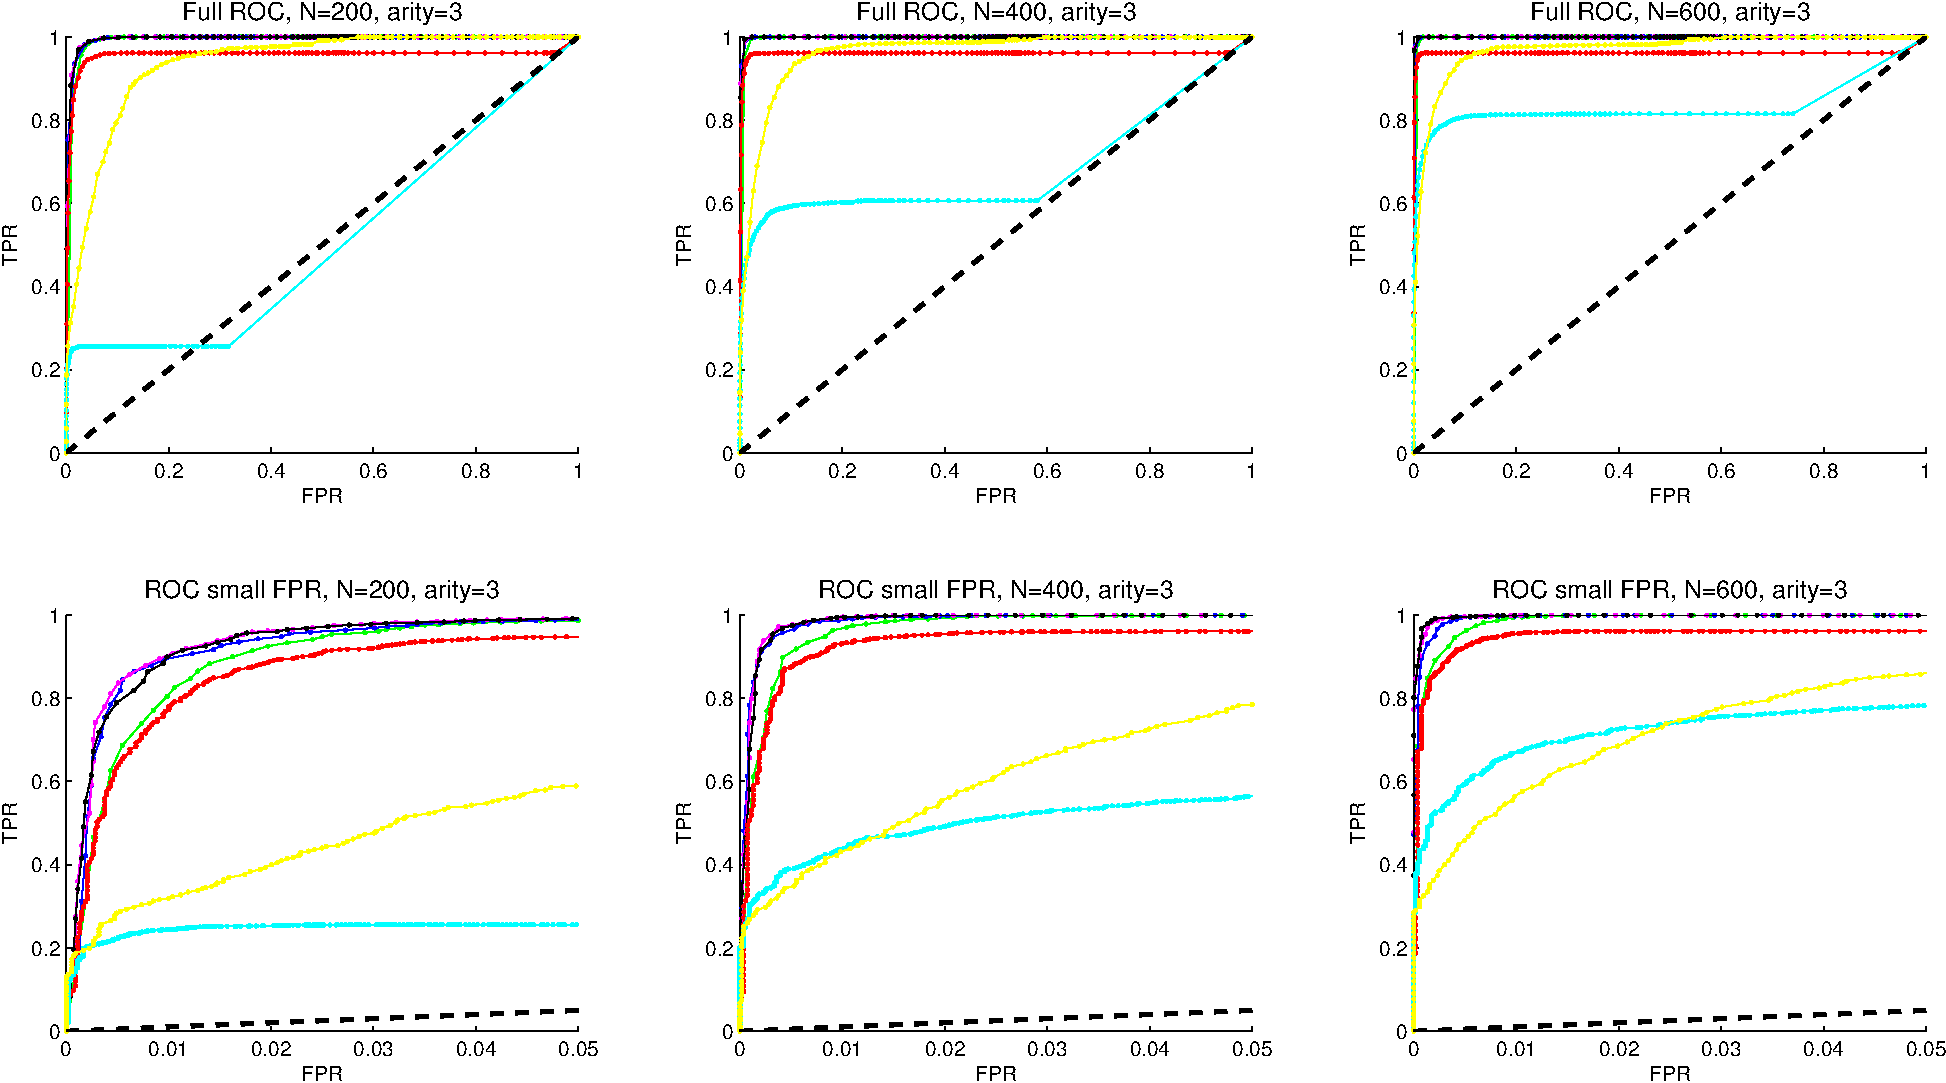
\includegraphics[width=0.45\linewidth]{img/linear_arity_3-eps-converted-to-crop.pdf} 
    }
    \quad
    \subfigure{
      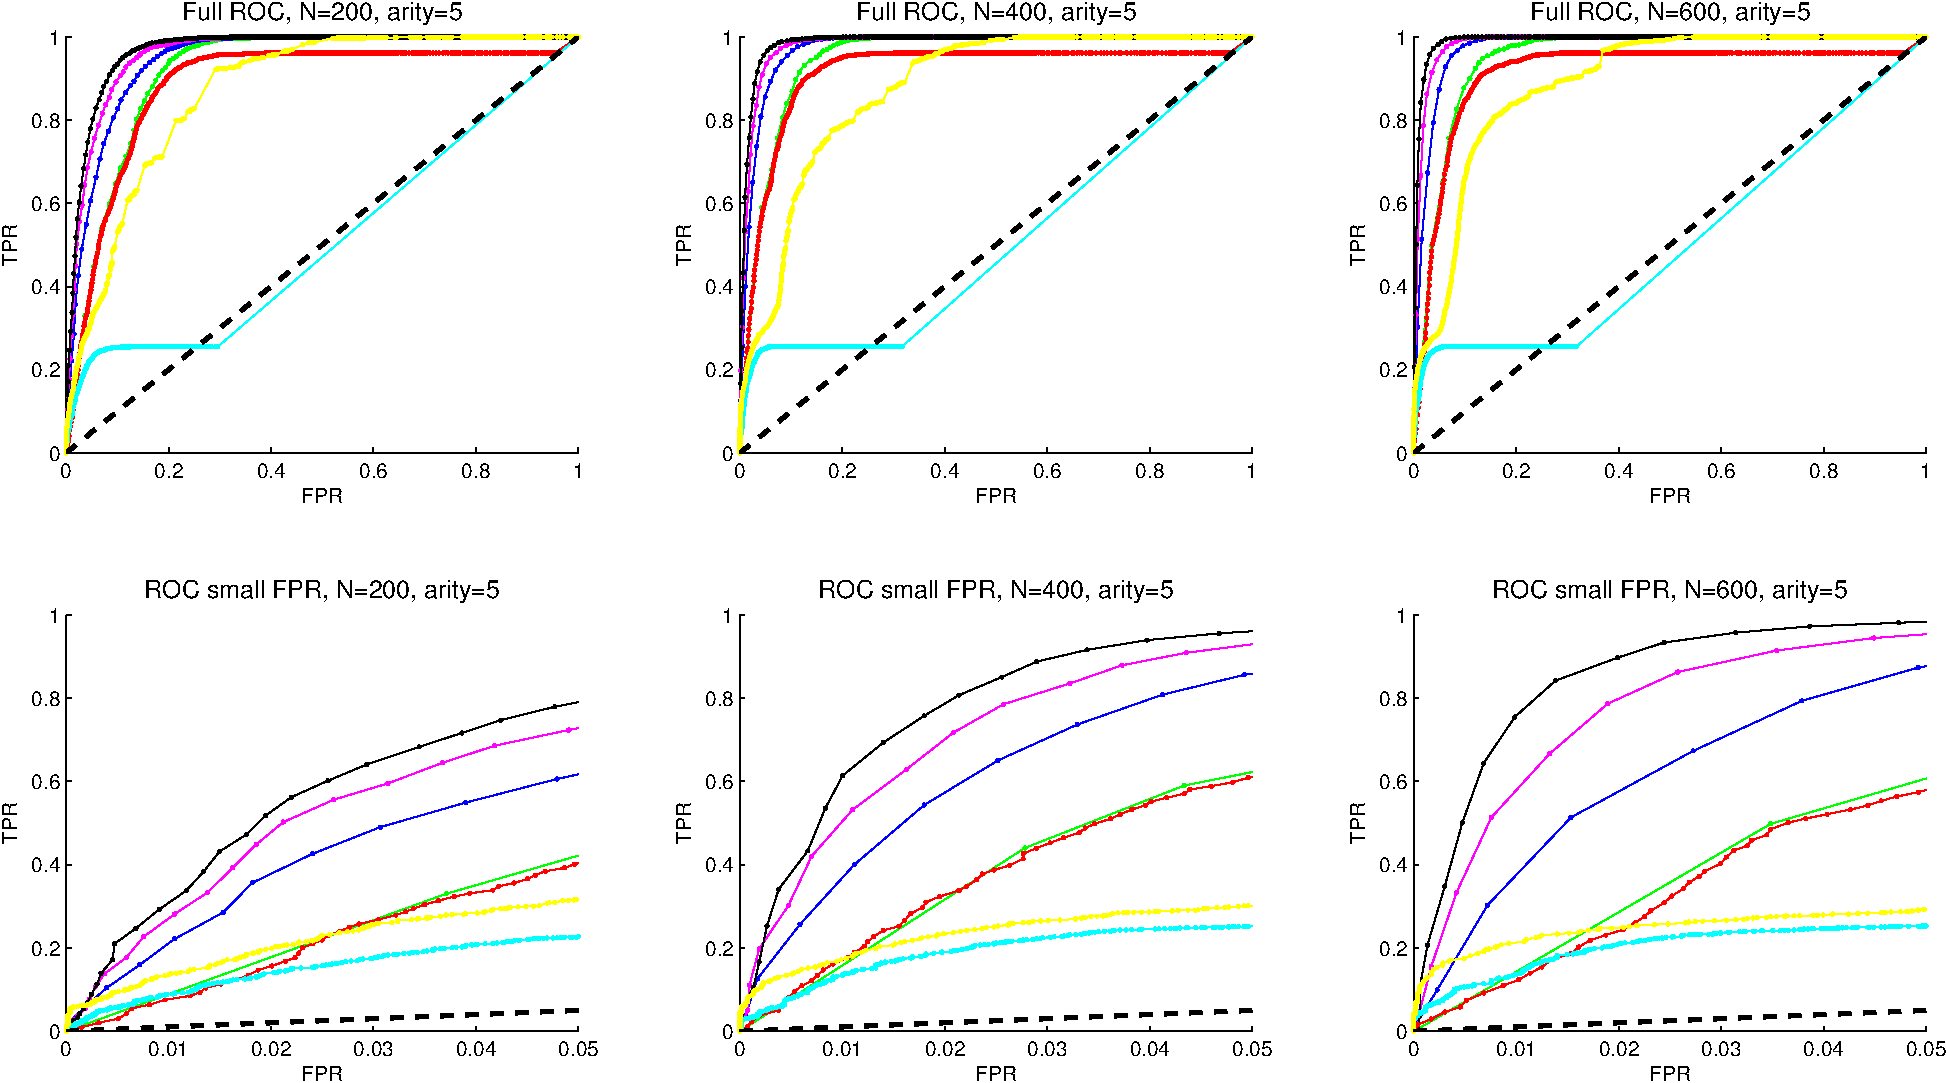
\includegraphics[width=0.45\linewidth]{img/linear_arity_5-eps-converted-to-crop.pdf} 
    }
\caption{ROCs for joint distributions generated from ``asia'' network structure with each variable having {\bf (Left)} arity 3, {\bf (Right)} arity 5, and each CPD with randomly sampled entries from $|\mathcal{N}(0, 1)|$, with a constant added along the diagonal of the CPD tensor (adding linear structure).}
\label{fig:asia_linear}
\end{figure}


\begin{figure}[h]
\centering
    \subfigure{
      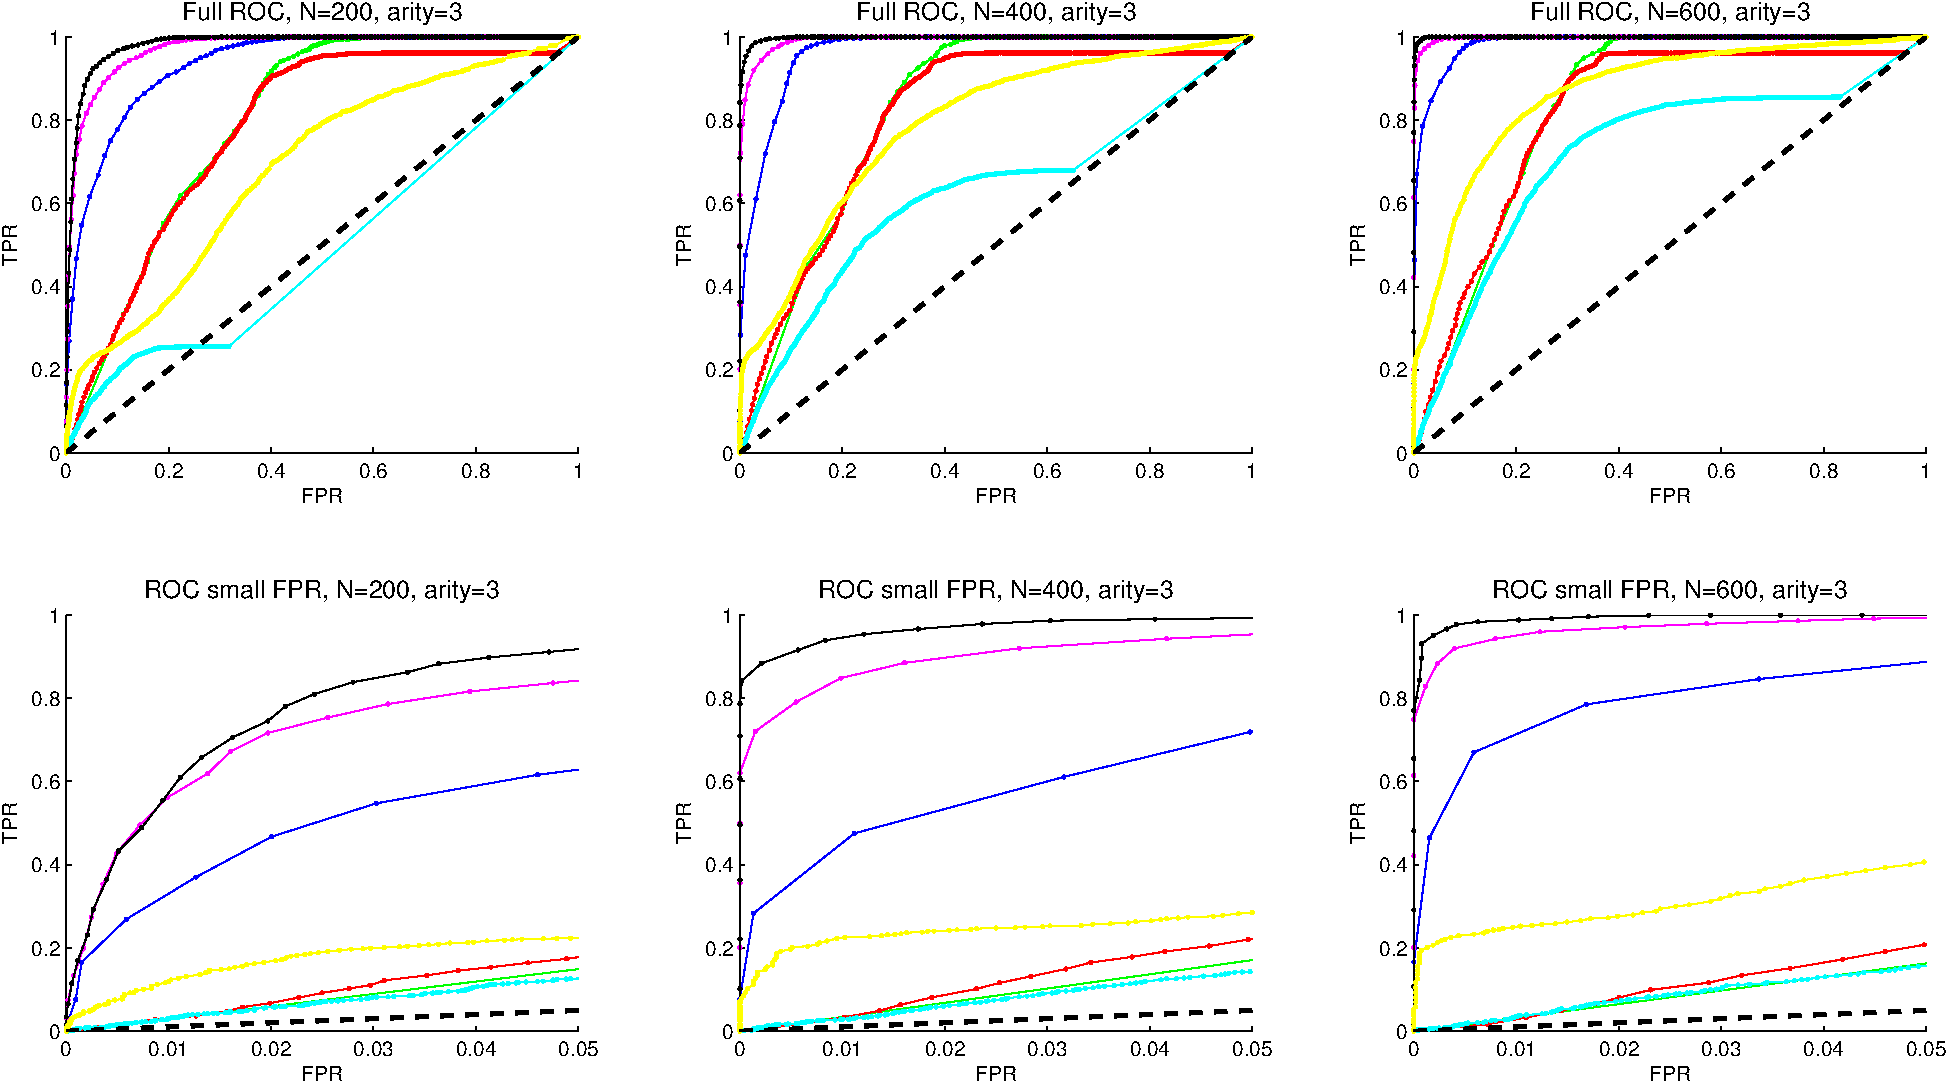
\includegraphics[width=0.45\linewidth]{img/random_arity_3-eps-converted-to-crop.pdf} 
    }
    \quad
    \subfigure{
      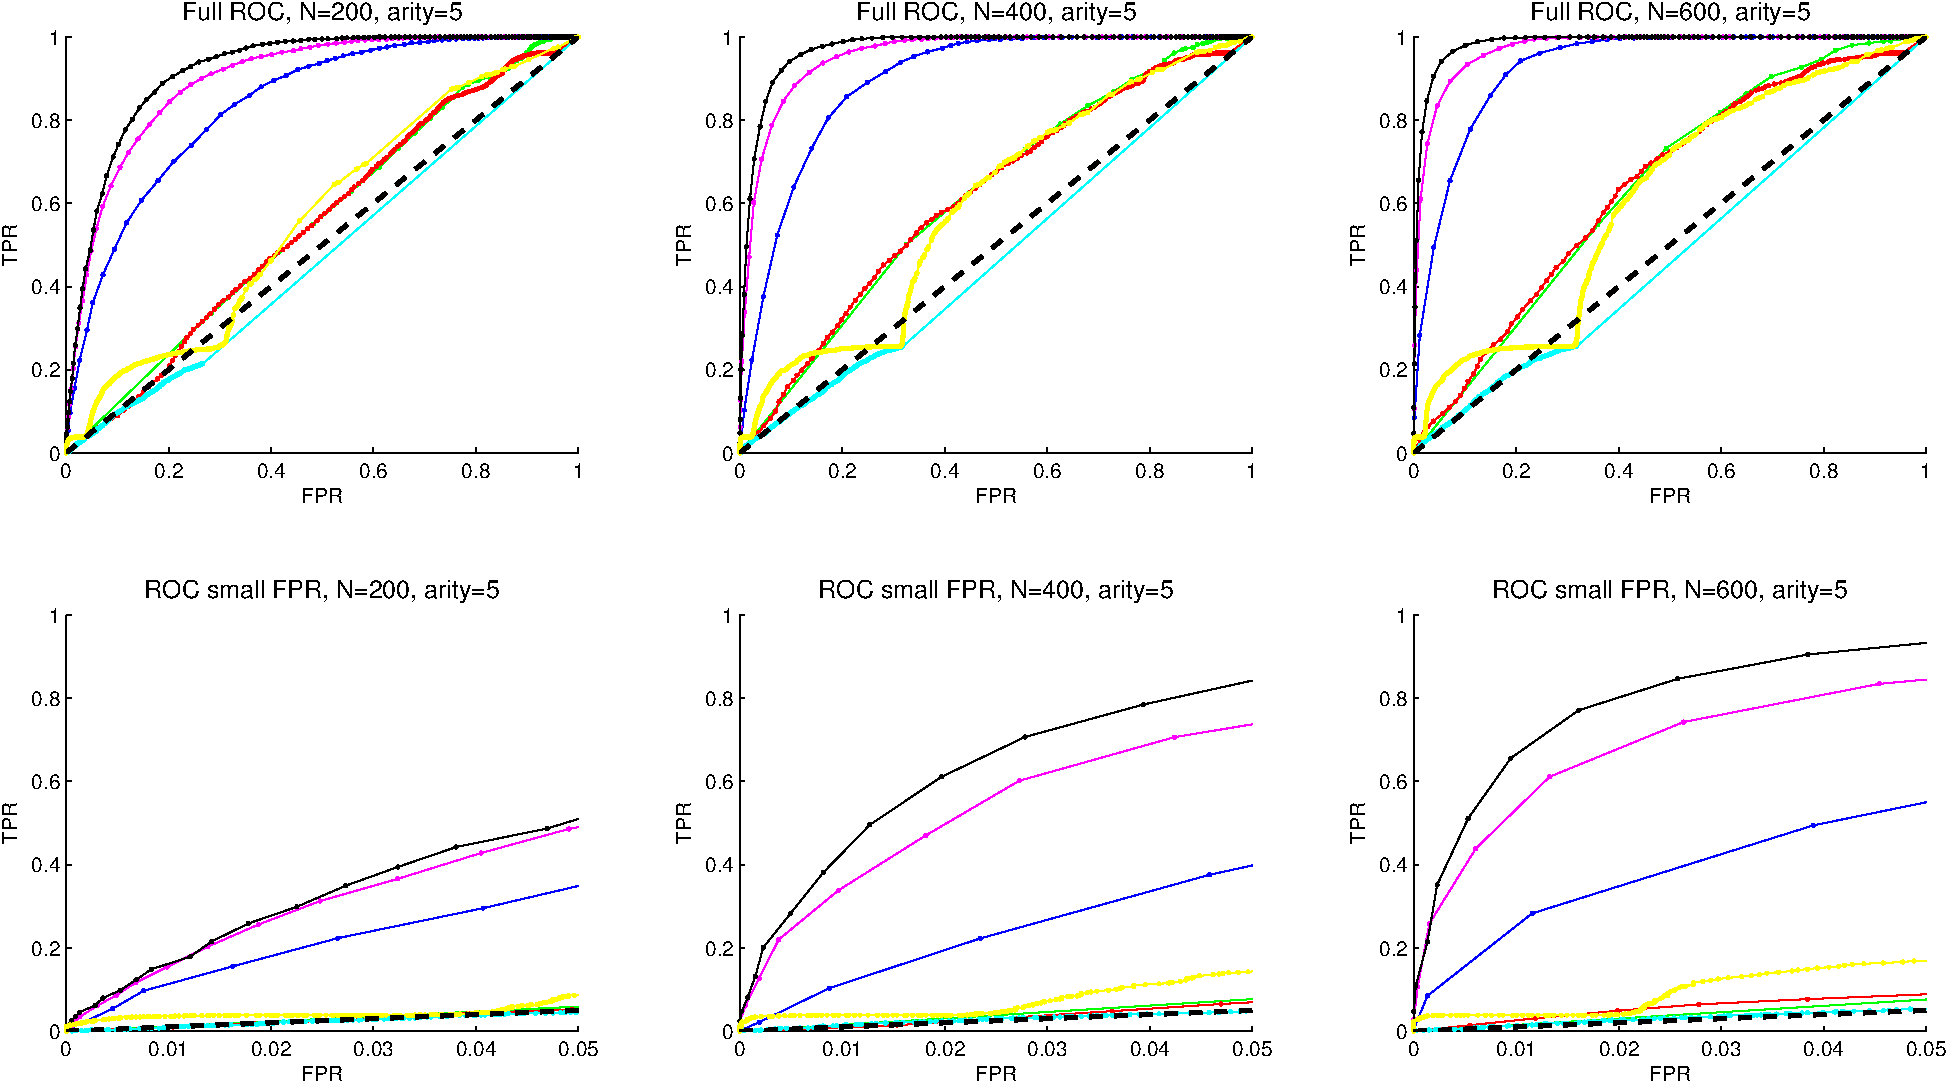
\includegraphics[width=0.45\linewidth]{img/random_arity_5-eps-converted-to-crop.pdf} 
    }
\caption{ROCs for joint distributions generated from ``asia'' network structure with each variable having {\bf (Left)} arity 3, {\bf (Right)} arity 5, and each CPD with randomly sampled entries from $|\mathcal{N}(0, 1)|$.}
\label{fig:asia_random}
\end{figure}

\subsection{Gene expression data}

\section{Discussion}

\begin{small}
%\renewcommand\bibname{References}
\bibliographystyle{abbrvnat}
%\bibliographystyle{authordate1}
%\bibliographystyle{amsnomr}
\bibliography{bibliography}
\end{small}

%\appendix
%\include{appendix}

\end{document}
